\documentclass[12pt]{article}
\setlength\parindent{0pt}
\usepackage{amsmath}
\usepackage{lscape}
\usepackage{graphicx}
\usepackage{fullpage}
\usepackage[margin=0.5in]{geometry}
\setlength{\parskip}{4mm}
\def\LL{\left\langle}   % left angle bracket
\def\RR{\right\rangle}  % right angle bracket
\def\LP{\left(}         % left parenthesis
\def\RP{\right)}        % right parenthesis
\def\LB{\left\{}        % left curly bracket
\def\RB{\right\}}       % right curly bracket
\def\PAR#1#2{ {{\partial #1}\over{\partial #2}} }
\def\PARTWO#1#2{ {{\partial^2 #1}\over{\partial #2}^2} }
\def\PARTWOMIX#1#2#3{ {{\partial^2 #1}\over{\partial #2 \partial #3}} }
\newcommand{\BE}{\begin{displaymath}}
\newcommand{\BC}{\begin{center}}
\newcommand{\EC}{\end{center}}
\newcommand{\EE}{\end{displaymath}}
\newcommand{\BNE}{\begin{equation}}
\newcommand{\ENE}{\end{equation}}
\newcommand{\BEA}{\begin{eqnarray}}
\newcommand{\EEA}{\nonumber\end{eqnarray}}
\newcommand{\EL}{\nonumber\\}
\newcommand{\la}[1]{\label{#1}}
\newcommand{\ie}{{\em i.e.\ }}
\newcommand{\eg}{{\em e.\,g.\ }}
\newcommand{\cf}{cf.\ }
\newcommand{\etc}{etc.\ }
\newcommand{\Tr}{{\rm tr}}
\newcommand{\etal}{{\it et al.}}
\newcommand{\OL}[1]{\overline{#1}\ } % overline
\newcommand{\OLL}[1]{\overline{\overline{#1}}\ } % double overline
\newcommand{\OON}{\frac{1}{N}} % "one over N"
\newcommand{\OOX}[1]{\frac{1}{#1}} % "one over X"
\pagenumbering{gobble}
\begin{document}
\Large
\centerline{\sc{Exercise -- Spectroscopy}}

\normalsize

\section{Types of Spectra}

In this exercise, you'll study how the interaction of light with atoms produces different sorts of spectra.

There are three kinds of spectra we need to understand:

\begin{enumerate}
	\item We already understand {\bf Continuous spectra}, which come from hot objects. Thermal radiation produces a continuous band of wavelengths, and so their spectra look like this:
	\BC
	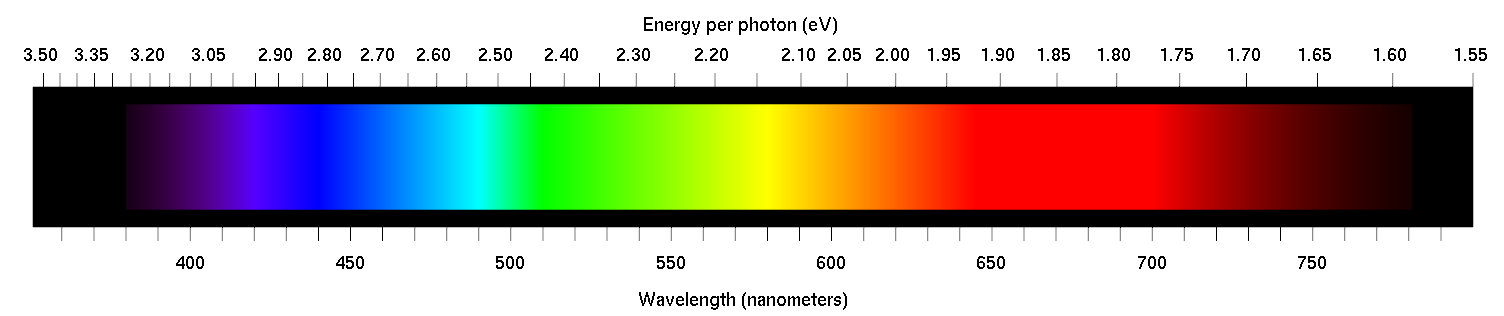
\includegraphics[width=4in]{spectrum-continuous.png}
	\EC
	
	
	
	
	\item {\bf Emission spectra}, which come from diffuse gases whose electrons are excited by electric current or extreme temperature. As their electrons transition back to the ground state, they emit light: photons of very specific energies equal to the {\it differences} between energy levels in the atoms that produced them.
	
	\BC
		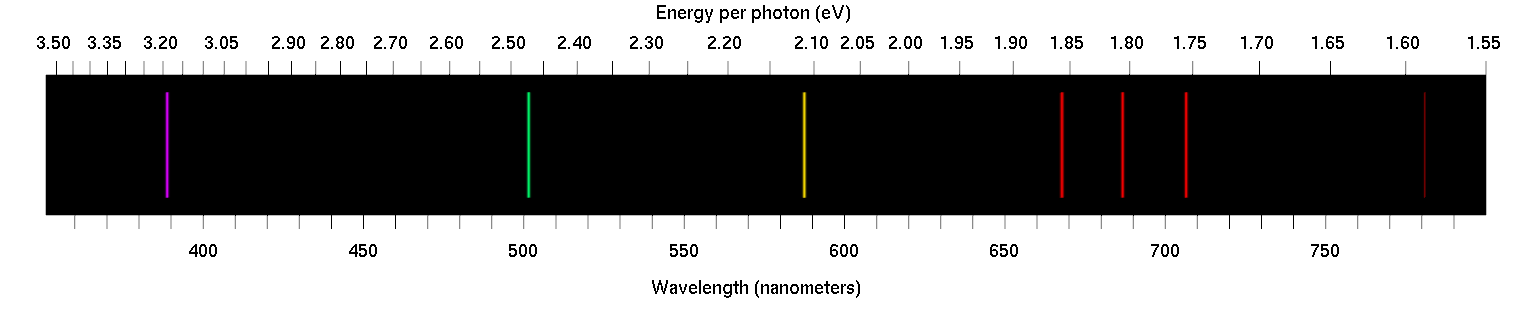
\includegraphics[width=4in]{spectrum-discrete.png}
	\EC
	\item {\bf Absorption spectra}, which come from hot objects viewed through an atmosphere. As a continuous spectrum passes through an atmosphere, each type of atom in that atmosphere absorbs the colors of light corresponding to the differences between its energy levels. This absorption removes those colors from the spectrum, leaving the rest behind. They look like this:
	\BC
	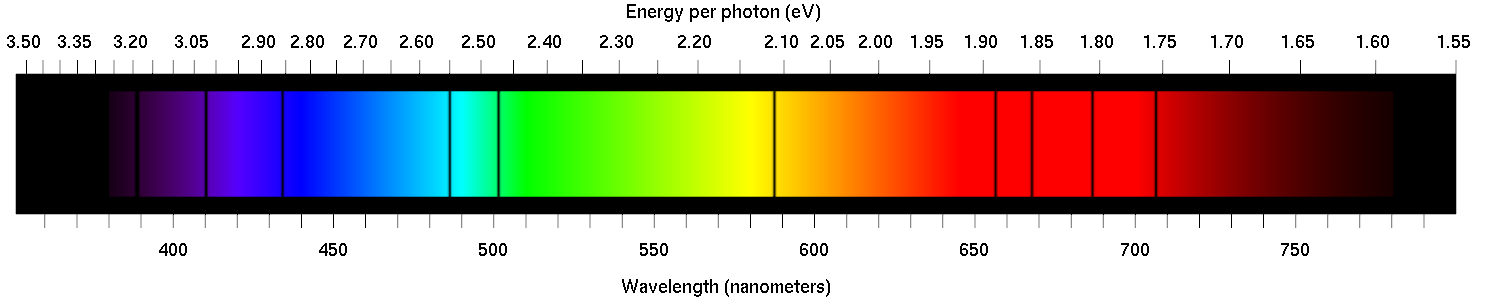
\includegraphics[width=4in]{spectrum-absorption.png}
	\EC
	
\end{enumerate}


Our goal here is to explore these last two types of spectra in detail. We'll use an example element called ``Orangium'', which has four energy levels as follows:

\begin{itemize}
	\setlength\itemsep{0in}
	\item $n=1$ with energy 0 eV (the ground state)
	\item $n=2$ with energy 3 eV 
	\item $n=3$ with energy 5 eV 
	\item $n=4$ with energy 5.5 eV 
\end{itemize}



\newpage

\section{Emission Spectra}


Draw an energy level diagram for this sort of atom below. Draw it to scale, so that (for instance) $n=3$ and $n=4$ are closer together than $n=1$ and $n=2$. 

\vspace{3in}

There are {\it six} possible transitions that atoms of this type can make. What are they? Fill out the chart below.

\begin{center}
	
	\Large

\begin{tabular}{|c|c|c|c|}
	\hline
	\normalsize Higher energy level &\normalsize Lower energy level & \normalsize Energy difference & \normalsize\hspace{1cm}Color\hspace{1cm} \\
	\hline
	& & & \\
	\hline
		& & & \\
	\hline
			& & & \\
	\hline
			& & & \\
	\hline
			& & & \\
	\hline
			& & & \\
	\hline
\end{tabular}
\end{center}

Do these transitions correspond to photons that orangium atoms could {\bf absorb}, photons that orangium atoms could {\bf emit}, or both? Explain why; if your answer is ``both'', explain what process causes absorption and what process causes emission.

\newpage


If a tube of diffuse orangium gas is excited by an electric current (like in a fluorescent light), the electrons will fall back down to the ground state, emitting photons whose energies are equal to the differences you found on the previous page. 

In the blank spectrum below, draw the lines that you would see, and label each one with the transition that produces it (e.g. $3 \rightarrow 2$).

\BC
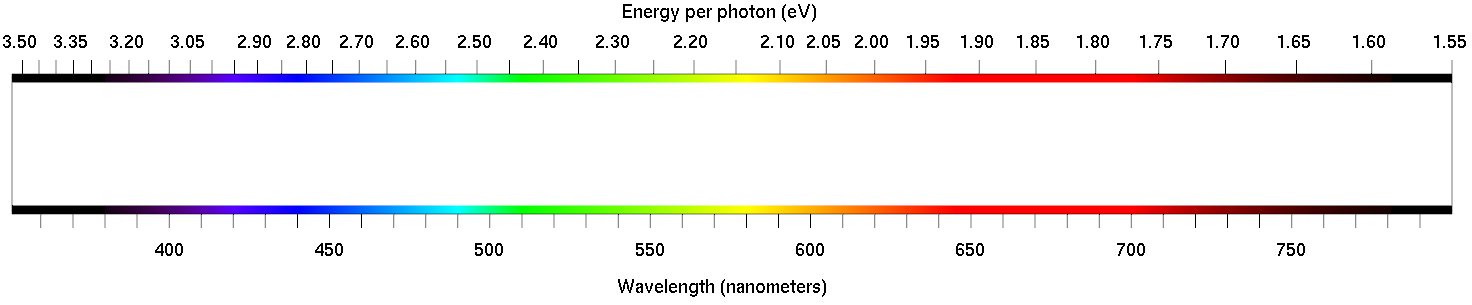
\includegraphics[width=7in]{spectrum-blank.png}
\EC

Would these be bright lines that appear on a dark background, or dark lines on a bright background? How do you know?

\vspace{1.2in}

\section{Absorption Spectra}

Imagine what happens when a hot object like the Sun shines through a thick cloud of orangium gas. As with any source of thermal radiation, its spectrum is continuous; it contains all colors of the rainbow: photons of all energies that we can see (and many energies that we can't see, not shown here).

As this light passes through the thick cloud of orangium, what would the orangium gas do to the 2 eV photons passing through it? Are there any other photons that would also behave in the same way?

\vspace{1in}

What would the orangium gas do to the 1.5 eV photons passing through it? What about 1.8 eV photons, or 3.14159 eV photons?

\vspace{0.5in}

\newpage


 The hot object would produce a spectrum that looks like this:

\begin{minipage}{0.15\textwidth}
	\begin{center}	\it Spectrum from\\
		hot object\end{center}
\end{minipage}
\begin{minipage}{0.8\textwidth}
	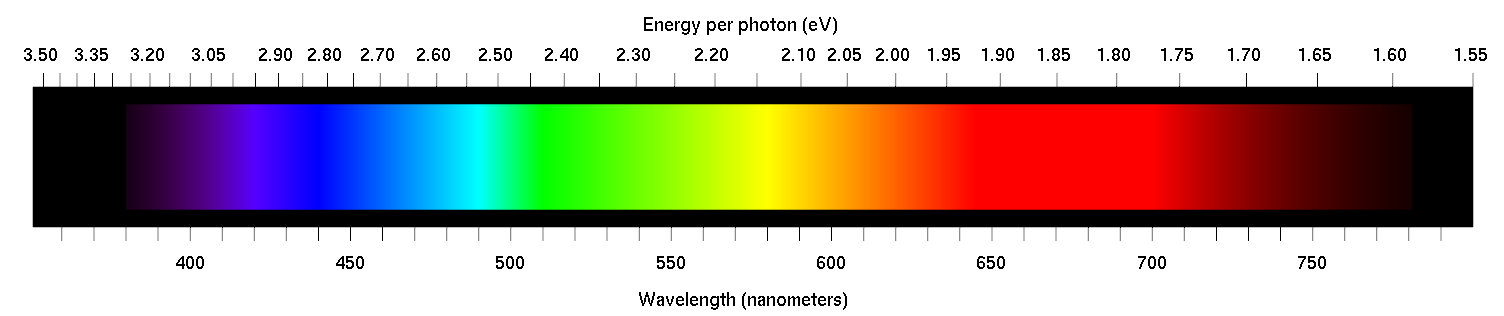
\includegraphics[width=5.5in]{spectrum-continuous.png}
\end{minipage}


What photon energies would be absorbed by the orangium? Draw them here.

\begin{minipage}{0.15\textwidth}
	\begin{center}	\it Colors absorbed\\
		by orangium\end{center}
\end{minipage}
\begin{minipage}{0.8\textwidth}
	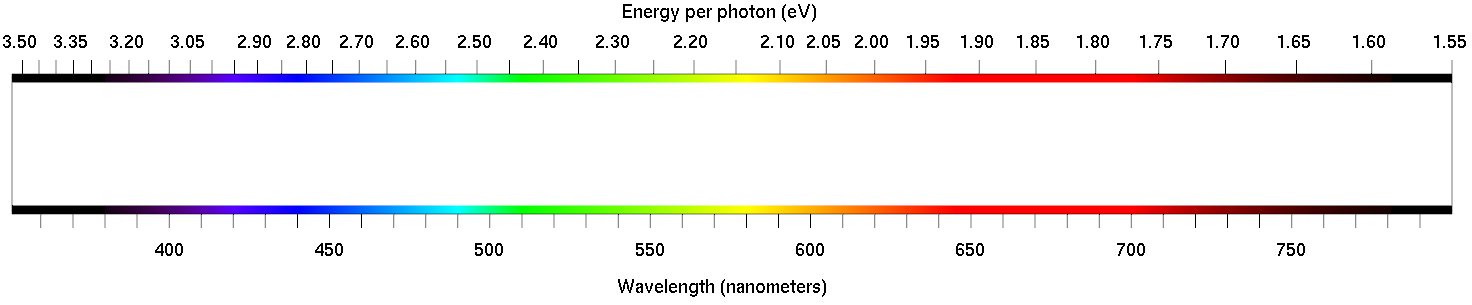
\includegraphics[width=5.5in]{spectrum-blank.png}
\end{minipage}

Draw the spectrum that would be left over afterwards below. {\bf Hint:} your pencils and pens make black marks on paper, and black is the absence of light...

\begin{minipage}{0.15\textwidth}
	\begin{center}	\it Resulting \\ spectrum\end{center}
\end{minipage}
\begin{minipage}{0.8\textwidth}
	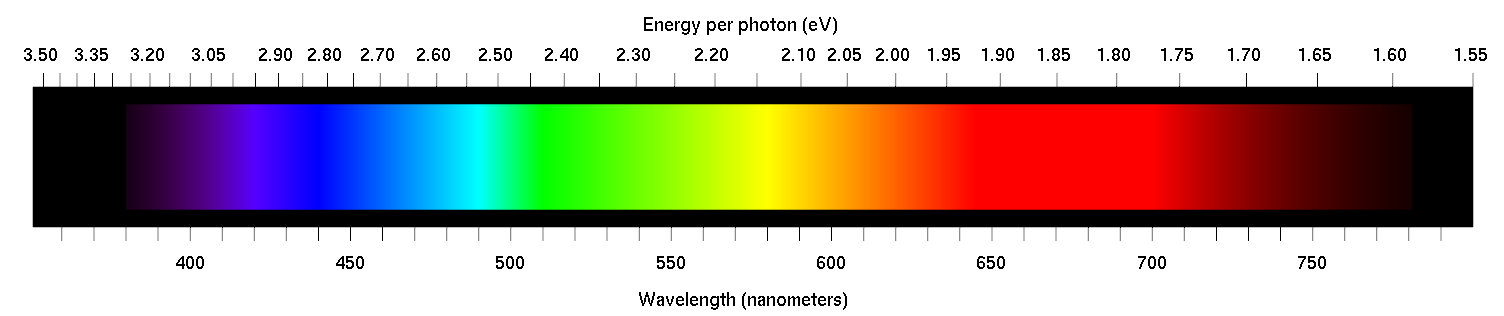
\includegraphics[width=5.5in]{spectrum-continuous.png}
\end{minipage}

\section{The Solar Spectrum}

What is the relation between the positions of the {\it bright} lines seen in the spectrum of an electrified tube of orangium gas and the positions of the {\it dark} lines seen in the spectrum when looking through a cloud of orangium?

\vspace{0.5in}

Suppose we saw dark lines at 2.00 eV, 2.50 eV, and 3.00 eV in the spectrum of the Sun. What could you conclude about the Sun's atmosphere?


\newpage

\centerline{\sc{\Large Homework 5 -- Spectroscopy}}
	
	\normalsize
	\begin{center}
		Due Thursday, November 3, by the end of class\\
		\small \it Note: You should finish this before Thursday's class; you may use it as part of your notes for the quiz.
	\end{center}
	
	\bigskip
	
	\begin{enumerate}
		
		
		\item Suppose a type of atom -- we'll call it onondagium -- has the following energy levels:
		\begin{itemize}
			\item $n=1$: 4 eV
			\item $n=2$: 6 eV
			\item $n=3$: 7.8 eV
			\item $n=4$: 9.5 eV
			\item $n=5$: 10 eV
		\end{itemize}
		
		If you put a diffuse gas of onondagium in a glass tube like the ones you've seen in class and lab and run an electric current through it, what would its spectrum look like? Draw the positions of any lines you would see, and tell whether they are bright lines on a dark background, or dark lines on a bright background. {\it (You will likely need a piece of scratch paper for this question.)}
		
		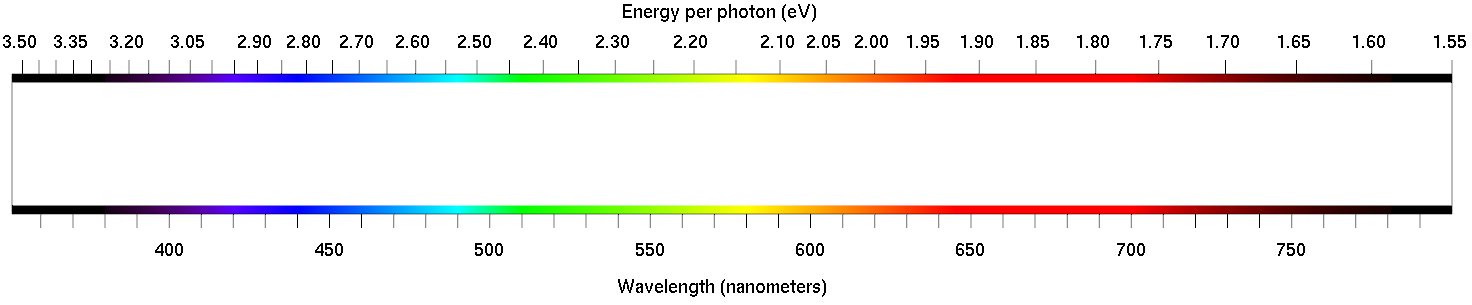
\includegraphics[width=7in]{spectrum-blank.png}
		\vspace{1in}
		
		Would your electrified tube of onondagium produce any spectral lines that you {\it cannot} see with your eye, but that you {\it could} detect with instruments? What energies would they have?
		
		\newpage
		
		
		\item Suppose a type of atom -- we'll call it syracusium -- has energy levels as follows:
		\begin{itemize}
			\item $n=1$: 0 eV (ground state)
			\item $n=2$: 2.1 eV
			\item $n=3$: 3 eV
			\item $n=4$: 5 eV
			\item $n=5$: 9 eV
		\end{itemize}
		
		Suppose now that you soak a piece of paper in syracusium and illuminate it with 5 eV photons. What would you see with your eye, if anything? 
		
		\vspace{1.3in}
		
		\item Forensic scientists sometimes use ``black lights'' -- lights that predominantly produce ultraviolet light-- in investigations. This UV light is not visible to our eyes, but when it shines on certain compounds 
		(such as blood), they glow with visible light. What is likely going on here, in light of the last problem? (That problem gives an example of how this might work -- remember 5 eV is in the ultraviolet.)
		
		\vspace{1.3in}
		
		\item Describe in a few sentences, in your own words, how the dark lines in the Sun's spectrum tell us what the Sun is made of.
		
		\vspace{2in}
		
		\it
		
		Your quiz on this will be at the end of class Thursday, November 3. This quiz will have three questions, as follows:
		
		\begin{itemize}
						\item I will ask you to determine the position of the spectral lines in the spectrum of an element with a given set of energy levels
						\item I will describe an object that emits light and ask what sort of spectrum (continuous, bright-line, or dark-line) that it would exhibit
			            \item I will ask you Question 4 from the homework, verbatim. (You can prepare your answer ahead of time, or copy it from your homework, but it must be in {\bf your own words}, not someone else's.)
		\end{itemize}
	\end{enumerate}
\end{document}

